%!TeX program = xelatex
\documentclass[12pt,hyperref,a4paper,UTF8]{ctexart}
\usepackage{UCASReport}
\usepackage{booktabs}
\usepackage{longtable}
\usepackage{array}
\usepackage{listings} % 加载 listings 包
\usepackage{color}
\usepackage[linesnumbered,ruled,vlined]{algorithm2e}
\usepackage{listings} 
\usepackage{float}

\definecolor{dkgreen}{rgb}{0,0.6,0}
\definecolor{gray}{rgb}{0.5,0.5,0.5}
\definecolor{mauve}{rgb}{0.58,0,0.82}

\lstset{ %
  language=Octave,                % the language of the code
  basicstyle=\footnotesize,           % the size of the fonts that are used for the code
  numbers=left,                   % where to put the line-numbers
  numberstyle=\tiny\color{gray},  % the style that is used for the line-numbers
  stepnumber=2,                   % the step between two line-numbers. If it's 1, each line 
                                  % will be numbered
  numbersep=5pt,                  % how far the line-numbers are from the code
  backgroundcolor=\color{white},      % choose the background color. You must add \usepackage{color}
  showspaces=false,               % show spaces adding particular underscores
  showstringspaces=false,         % underline spaces within strings
  showtabs=false,                 % show tabs within strings adding particular underscores
  frame=single,                   % adds a frame around the code
  rulecolor=\color{black},        % if not set, the frame-color may be changed on line-breaks within not-black text (e.g. commens (green here))
  tabsize=2,                      % sets default tabsize to 2 spaces
  captionpos=b,                   % sets the caption-position to bottom
  breaklines=true,                % sets automatic line breaking
  breakatwhitespace=false,        % sets if automatic breaks should only happen at whitespace
  title=\lstname,                   % show the filename of files included with \lstinputlisting;
                                  % also try caption instead of title
  keywordstyle=\color{blue},          % keyword style
  commentstyle=\color{dkgreen},       % comment style
  stringstyle=\color{mauve},         % string literal style
  escapeinside={\%*}{*)},            % if you want to add LaTeX within your code
  morekeywords={*,...}               % if you want to add more keywords to the set
}

%%-------------------------------正文开始---------------------------%%
\begin{document}

%%-----------------------封面--------------------%%
\cover

%%------------------摘要-------------%%
%\begin{abstract}
%
%在此填写摘要内容
%
%\end{abstract}

\thispagestyle{empty} % 首页不显示页码

%%--------------------------目录页------------------------%%
\newpage
\tableofcontents

%%------------------------正文页从这里开始-------------------%
\newpage

%%可选择这里也放一个标题
%\begin{center}
%    \title{ \Huge \textbf{{标题}}}
%\end{center}
\section{摘要}
\section{研究背景}
信息技术的迅猛发展引领人类社会迈向信息化与智能化新时代,数据呈指数级增长。此背景下,自然语言处理(NLP)作为人机沟通的纽带,其重要性与日俱增。从计算机科学分支跃升至发掘非结构化文本数据潜能、促信息处理高效化和智能化的核心技术,NLP的发展伴随互联网、社交媒体、数字文献等产生的海量数据激增及计算能力建设的飞越,实现了前所未有的技术突破与应用拓宽。

汉语文本处理中,多音字与易错字构成重大障碍。手工筛查耗时且难以保证准确,尤其在大规模文档中,效率与精确性两难求解,愈发突显自动化处理工具的迫切需求。

与此同时,人工智能技术,特别是深度学习领域的飞速进步,如深度神经网络的广泛部署,极大地增强了机器理解和处理自然语言的能力。这些进展不仅仅优化了语音识别、机器翻译等领域,亦为解决自动标注汉字读音等细粒度任务铺平了道路,展现了技术在特定应用场景中的实用性与潜力。
\section{研究动机}
本文旨在利用自然语言处理技术,实现对Word文档中多音字与易错字的自动标注。通过构建多音字与易错字的标注模型,实现对文档中多音字与易错字的自动标注,提高文档处理效率,减少人工标注工作量。
研究动机分为以下两个方面:
\subsection{实际生活需求}
自动注音系统的研发,其首要动机在于解决现实生活中的实际问题,提高人们处理文本的准确性和效率。在演讲准备、教材制作、语言教学、有声书录制等领域,自动为文档加上正确的注音能够显著降低错误发生率,确保发音准确无误,如演讲者念稿时避免误读多音字,确保传达的信息清晰无误。这不仅提升了交流的专业度,还增强了信息接收者的理解体验,使得语言文化传播更为流畅和准确。

此外,在教育、科学研究、新闻媒体、法律、医疗健康等领域,文档处理需求日益增长,对文档内容的准确性和专业性提出更高要求。然而,由于汉语的独特性质,如一字多音、同音异义现象的存在,使得中文文档处理面临特别的挑战。手动校对多音字和易错字费时费力,特别是在处理大规模文档时,效率和准确性难以保障。这种情况下,自动化文本处理工具的需求显得尤为迫切。

为了便于实际使用,我组成员还设计了用户交互界面,使得用户可以方便地上传文档,即使不会写任何程序,也可以轻松地使用我们的系统进行多音字的自动注音。
\subsection{学生能力培养}
通过这个项目,我们能够将课堂上学到的自然语言处理理论知识与实际问题解决结合起来,加深了对NLP技术本质的理解,如词法分析、语义理解、机器学习模型等概念不再是抽象的文字,而是变成了具体实现代码和技术选型的决策过程。通过处理多音字和易错字的注音任务,我们能够更好地掌握汉语语言特性与语法规则,从而加深对汉语语言学的理解。这个过程需要我们不断思考如何在复杂的语言环境中精确识别多音字的读音,并通过各种算法策略进行纠错。这不仅提升了我们的理论知识,还增强了在实际应用场景中灵活运用所学知识的能力。

在项目的实践中,我们有机会接触到多种NLP技术,例如分词、词性标注、语音合成等。
我们使用python和pytorch编写程序,git进行代码协作与管理,提升了团队成员之间的协作能力,也让我们在编程技能和工程实践上得到了很大的提升。
每个阶段的方案讨论和调整,都是对我们逻辑思维、问题分析和解决能力的综合考验。

此外,这个作业让我们更深入地体会到了科研的严谨性与创新性。为了实现高精度的注音功能,我们需要广泛查阅文献,
分析现有的多音字处理方案,并训练了自己的模型。在这个过程中,我们不仅学会了如何全面理解一个研究问题,
还培养了在面对复杂问题时,能够从多角度提出创新性解决方案的能力。为使工具易于使用且效果直观,在ui界面时我们不得不站在用户的角度思考,
提升了我们的产品设计思维。
\section{技术路线}
\subsection{方法一:使用pypinyin库}
python-pinyin是一个用于将汉字转换为拼音的python库,其开源地址为\url{https://github.com/mozillazg/python-pinyin}。它支持多种拼音风格,包括声调和无声调。我们可以使用它来实现对文档中多音字的自动标注。
\begin{lstlisting}
    >>> from pypinyin import pinyin, lazy_pinyin, Style
    >>> pinyin('中心')  # or pinyin(['中心']),参数值为列表时表示输入的是已分词后的数据
    [['zhōng'], ['xīn']]
    >>> pinyin('中心', style=Style.TONE2, heteronym=True)
    [['zho1ng', 'zho4ng'], ['xi1n']]
    >>> lazy_pinyin('中心')  # 不考虑多音字的情况
    ['zhong', 'xin']
    >>> lazy_pinyin('战略', v_to_u=True)  # 不使用 v 表示 ü
    ['zhan', 'lüe']
\end{lstlisting}
\begin{algorithm}[H]
    \caption{使用pypinyin库实现对word文档中多音字的自动标注}
    \KwIn{原word文档, 多音字字库 \texttt{polyphone\_data}}
    \KwOut{注音后的word文档}
    
    \SetKwFunction{ReadWord}{ReadWord}
    \SetKwFunction{GetPinyinForRareCharacter}{GetPinyinForRareCharacter}
    \SetKwFunction{ProcessText}{ProcessText}
    \SetKwFunction{SaveWord}{SaveWord}
    
    \SetKwProg{Fn}{Function}{:}{}
    
    \BlankLine
    读取Word文档内容,获取文本段落 \textbf{paragraphs}\;
    \ForEach{paragraph \textbf{$\in$ paragraphs}}{
        \ForEach{character \textbf{$\in$ paragraph}}{
            \If{character \textbf{$\in$ polyphone\_data}}{
                添加多音字及其注音到输出段落\;
            }
            \Else{
                直接添加字符到输出段落\;
            }
        }
    }
    输出注音后的word文档\;
\end{algorithm}
\vspace{\baselineskip}
以下是部分核心代码展示:
\begin{lstlisting}
    def add_pinyin_to_polyphone_words(paragraphs, polyphone_data):
    polyphonic_chars = {item['char'] for item in polyphone_data}
    rare_chars = {item['char'] for item in rare_char_data}
    output_paragraphs = []

    for paragraph in paragraphs:
        pinyin_paragraph = pinyin(paragraph, style=Style.TONE)
        output_paragraph = ""
        char_index = 0
        for char in paragraph:
            if char in polyphonic_chars :
                output_paragraph += char + '(' + pinyin_paragraph[char_index][0] + ')'
            elif char in rare_chars:
                output_paragraph += char + '[' + get_pinyin(char)[0] + ']'
            else:
                output_paragraph += char
            char_index += 1
        output_paragraphs.append(output_paragraph)
    return output_paragraphs
\end{lstlisting}

\subsection{方法二:使用LSTM神经网络模型}
在本节中我们将简要介绍如何训练和使用LSTM模型进行多音字和难见字注音。
\subsubsection{数据集构建}
训练一个神经网络往往需要一个高质量的特定数据集,为了实现准确的多音字和难字注音目标,方法二主要利用了四类数据集,其中有些是我们自己构建的,而有些是我们直接引用前人构建的相关数据集,最后分别对不同数据集进行了简单的优势与不足分析。
\paragraph{一、爬虫+pypinyin库:(数据集构建的代码为 method2/get\_data.py)}%\_是转义字符
该项目主要分为以下几个步骤:
\begin{enumerate}
    \item \textbf{数据采集}:本项目使用了爬虫 + Pypinyin 库自动注音的方式获取了训练所需的多音字数据集。首先,我们使用爬虫技术从公开网站上获取某个月人民日报的中文文本数据,规模大约为两百万文字(3.7 MB)。爬取到的文本数据包含丰富的语料库,涵盖了多种语境下的多音字,适合作为中文多音字的训练集。我们通过对爬取的文本数据进行处理,并借助 Python 编程语言与Pypinyin相关库,自动为多音字添加拼音注释,最后构建出一个可以用于训练 LSTM 模型的标准化数据集。
    \item \textbf{数据预处理}:使用 Python 的正则表达式对爬取的文本进行清洗与分句处理。以下是部分核心代码展示:
  \begin{lstlisting}[caption={方法一数据预处理}, label={lst:example}]
      # 读取docx文件
      doc = Document('data/train_pinyin_file.docx')  # 替换为你的文件名
      # 遍历文档中的段落
      for para in doc.paragraphs:
          text = para.text
          # 使用标点符号分隔句子
          sentences = re.split(r'[。;,]', text)
  \end{lstlisting}
    \item \textbf{多音字匹配及拼音注音}:使用 pypinyin 库,我们可以自动为文本中的每个汉字生成拼音。对于多音字,我们会根据语境信息选择正确的发音并附加注音。对于每个句子,正则表达式 \texttt{r'(\textbackslash w+)((\textbackslash w+))'}被用来提取带有拼音的词语,并将其与句子中出现的多音字进行对应。同时为了保证数据多样性和合理性,每个多音字的相同拼音不会在数据集中重复出现超过 10 次。以下是部分核心代码展示:
  \begin{lstlisting}[caption={方法一多音字匹配及拼音注音}, label={lst:example}]
  for sentence in sentences:
      matches = re.findall(r'(\w+)((\w+))', sentence)
      for word, pronunciation in matches:
      # 清理句子中的注音部分
      cleaned_sentence = re.sub(r'\(.*?\)', '', sentence).strip()
      
      # 判断该多音字及其拼音是否已在数据集中存在
      if word in train_data:
          existing_pronunciations = [entry[2] for entry in train_data[word]]
          if existing_pronunciations.count(pronunciation) > 10:
              continue  # 跳过发音已存超过 5 次的条目
      
      # 只处理单个汉字的多音字
      if len(word) > 1:
          continue
  
      # 将新词条加入数据集
      if word not in train_data:
          train_data[word] = []
      train_data[word].append((cleaned_sentence, word, pronunciation))
  \end{lstlisting}
  \item \textbf{数据集存储}:在数据集中,每个汉字的拼音都会与它所在的句子一起保存,确保上下文信息不丢失。我们为每个多音字构建一个包含句子、拼音和汉字的结构化条目,存储到 JSON 文件中,形成训练数据集,数据结构如下所示:
  
  
  % 创建高亮文本框
  \begin{tcolorbox}
    "了": [\\
      ('他已经回来了', '了', 'le'),\\
      ('你去了哪里?', '了', 'le'),\\
      ('事情终于结束了', '了', 'le'),\\
      ('我吃完饭了', '了', 'le'),\\
      ('他笑了起来', '了', 'le'),\\
      ('问题解决了', '了', 'le'),\\
      ('我早就知道了', '了', 'le'),\\
      ('那件事了了', '了', 'liǎo'),\\
      ('他什么都不明了', '了', 'liǎo'),\\
      ('事情很快了结', '了', 'liǎo'),\\
      ],
  \end{tcolorbox}
  \end{enumerate}
  \paragraph{二、大模型构建数据集}
  \indent 随着深度学习技术的飞速发展,大型预训练模型(Large Language Models, LLMs)如GPT系列、BERT等在自然语言处理(NLP)领域取得了显著成就。然而,为了进一步微调模型以适应特定任务,往往需要高质量的领域数据集,因此本文高效地利用大语言模型来构建多音字数据集。\\
  \indent 通过大模型自动构建数据集需要进行prompt设计,并在prompt结合样例,即让大模型进行少样本学习(few shot learning)。prompt样例如下所示:
  % 创建高亮文本框
  \begin{tcolorbox}
    '六': ('liù', 'lù'), '切': ('qiē', 'qiè'), '分': ('fēn', 'fèn'),... 请为这些多音字,每个字生成 10 个句子,样式为: "少": [ ("少年的时光很宝贵", "少", "shào"), ("少数服从多数是原则", "少", "shǎo"), ("少林寺的武功很厉害", "少", "shào"), ("他少言寡语", "少", "shǎo"), ("少年强则国强", "少", "shào"), ("少部分人持有异议", "少", "shǎo"), ("他少不更事", "少", "shào"), ("少安毋躁,慢慢来", "少", "shǎo"), ("少年的志向很远大", "少", "shào"), ("少一点抱怨,多一点行动", "少", "shǎo") ], 
  \end{tcolorbox}
  \indent 尽管大语言模型具有很强的语言理解和生成能力,但不可避免地会出现幻觉现象,生产错误的注音样例,如下为两个错误输出样例:

\begin{figure}[htbp]
    \centering
    \begin{minipage}[b]{0.45\textwidth}
        \centering
        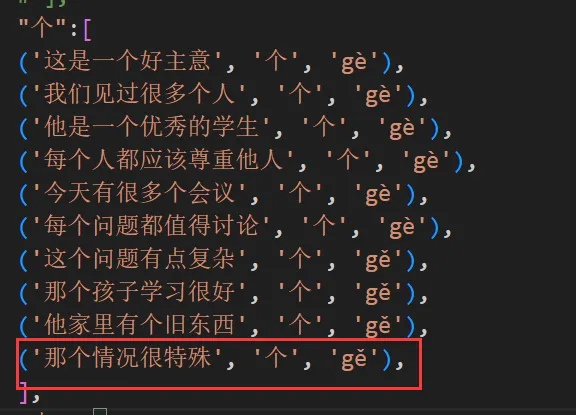
\includegraphics[width=\textwidth]{figures/image.png} % 替换为第一张图片的路径
        \caption{大模型生成错误样例1}
        \label{fig:image1}
    \end{minipage}
    \hspace{0.05\textwidth} % 两张图片之间的水平间隔
    \begin{minipage}[b]{0.45\textwidth}
        \centering
        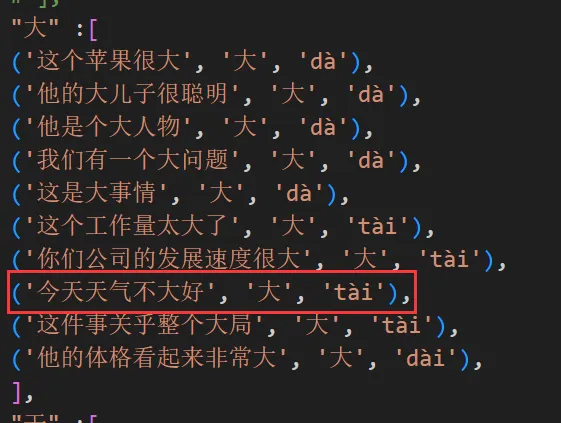
\includegraphics[width=\textwidth]{figures/image1.png} % 替换为第二张图片的路径
        \caption{大模型生成错误样例2}
        \label{fig:image2}
    \end{minipage}
\end{figure}
\paragraph{三、使用 train.csv 数据集 + 人工处理}
\indent 我们在GitHub上(\url{https://github.com/Jackiexiao/tts-frontend-dataset})下载了开源数据集train.csv,然后处理利用正则表达式实现拼音提取与文字提取,同时为了保障训练数据的多样性,我们平衡了每个读音样例的数量。 (实际中相同的发音可能限制最多 10 个或20个),如下图所示:
\begin{figure}[H]%通过引入 float 包,可以使用 [H] 参数强制图片出现在当前位置。
    \centering
    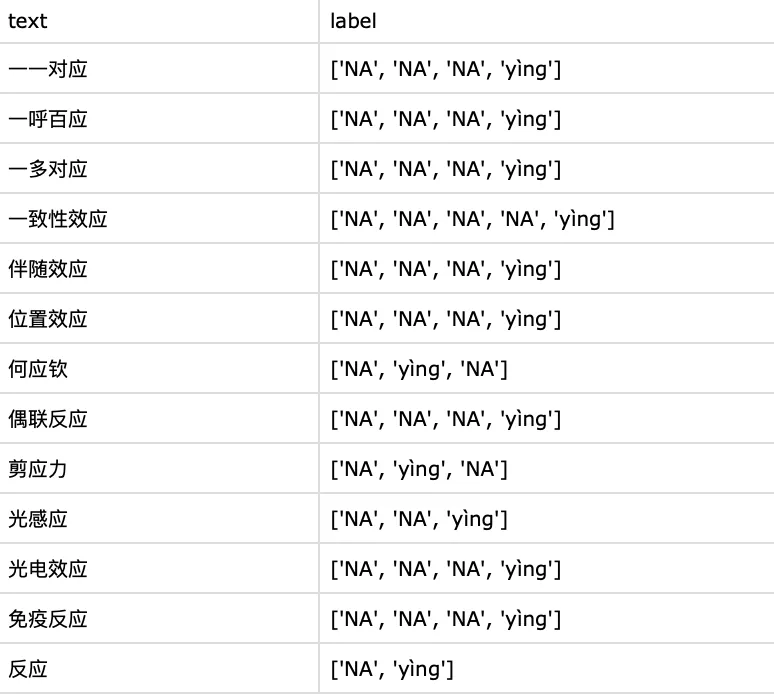
\includegraphics[width=0.5\linewidth]{figures/image2.png}
    \caption{train.csv数据集样例}
    \label{fig:enter-label}
\end{figure}
\paragraph{四、使用论文中开源数据集}
我们参考了论文《CVTE-Poly: A New Benchmark for Chinese Polyphone Disambiguation》,并从\url{https://github.com/NewZsh/polyphone} GitHub仓库中下载了训练数据集,分别为train big.sent和train big.lb两个文件,前者为训练文本数据,后者训练文本对应的多音字注音数据,并利用两个下划线标记了需要注音的字。s数据格式如下图所示:
\begin{figure}[htbp]
    \centering
    \begin{minipage}[b]{0.45\textwidth}
        \centering
        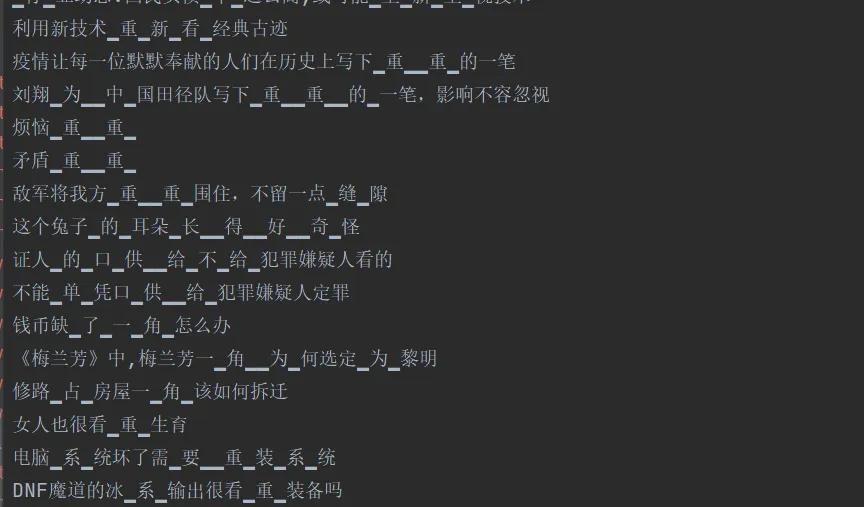
\includegraphics[width=\textwidth]{figures/image3.png} % 替换为第一张图片的路径
        \caption{train big.sent}
        \label{fig:image3}
    \end{minipage}
    \hspace{0.05\textwidth} % 两张图片之间的水平间隔
    \begin{minipage}[b]{0.45\textwidth}
        \centering
        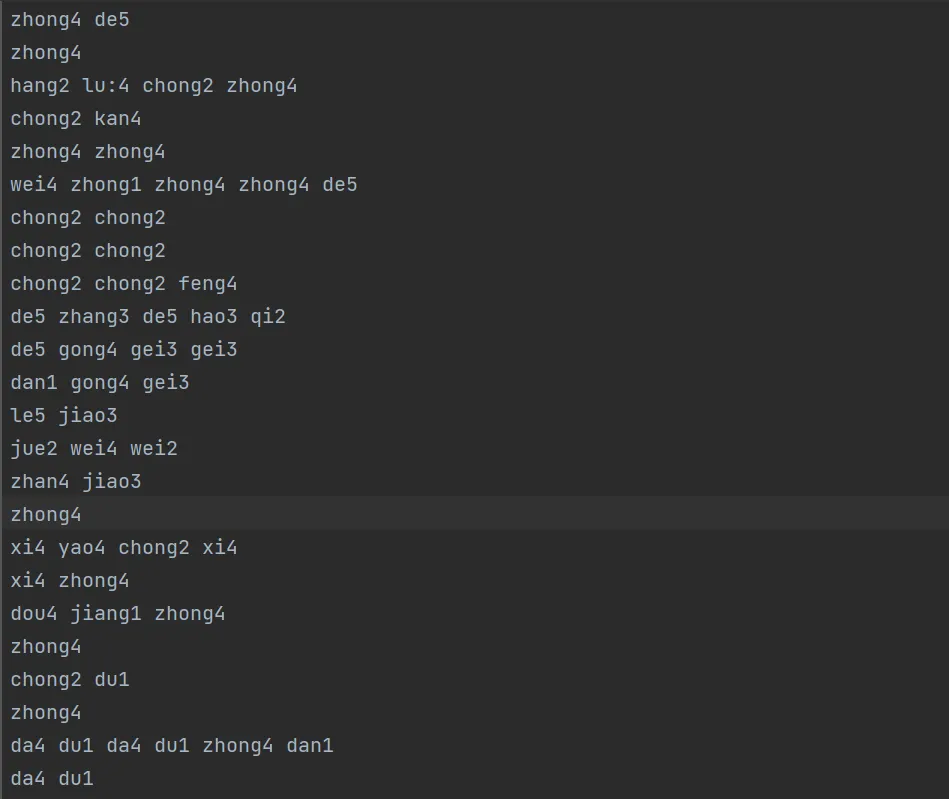
\includegraphics[width=\textwidth]{figures/image4.png} % 替换为第二张图片的路径
        \caption{train big.lb }
        \label{fig:image4}
    \end{minipage}
\end{figure}
\subsubsection{DisambiguationLSTM神经网络模型}
在训练过程中,该方法利用了DisambiguationLSTM神经网络模型,每个网络是一层 Embedding + LSTM,并为每个字(word)训练一个 DisambiguationLSTM , 然后使用 nn.ModuleDict 的方式做模型集成,最后在测试阶段,测试集中的每个词都可以使用对应的模型做推理,模型实现代码细节如下:
\begin{lstlisting}[caption={DisambiguationLSTM神经网络模型实现代码}, label={lst:example}]
class DisambiguationLSTM(nn.Module):
    def __init__(self, n_word, word_dim, word_hidden, n_pronounce):
        super(DisambiguationLSTM, self).__init__()
        self.word_embedding = nn.Embedding(n_word, word_dim)
        self.lstm = nn.LSTM(input_size=word_dim, hidden_size=word_hidden, batch_first=True, bidirectional=True)
        self.linear1 = nn.Linear(word_hidden*2, n_pronounce)
    def forward(self, x):
        x = self.word_embedding(x)
        x = x.unsqueeze(0)      # x.size() : (1,5,100)
        x, _ = self.lstm(x)     # x.size(): (1,5,256)
        x_out = x[:, -1, :]     # 全连接层的输入为神经网络最后一层最后一个time step的输出
        x = self.linear1(x_out)     # x.size() : (1,2)
        return x  详细解释一下这个网络的原理
\end{lstlisting}
这个 DisambiguationLSTM 是一个基于 PyTorch 的 LSTM(长短期记忆网络)模型,专门用于处理序列数据。以下是对该模型的详细解释:
\begin{enumerate}
  \item \textbf{Embedding 层 (self.word\_embedding):}
  \begin{itemize}
  \item 作用:将输入的单词序列转换成低维的稠密向量表示,通常称为“词嵌入”。
  \item 每个单词在词汇表中的索引,维度为 (batch\_size, sequence\_length),即每一行表示一个句子或单词序列。
  \item 输出:将每个索引转换成一个 word\_dim 维度的向量,输出的维度为 (batch\_size, sequence\_length, word\_dim),即每个单词被转换成一个 word\_dim 维的向量。
\end{itemize}
  \item \textbf{LSTM 层 (self.lstm):}
  \begin{itemize}
  \item 作用:LSTM 是一种特殊的循环神经网络(RNN),能够捕捉序列数据中的长期依赖关系。它通过“记忆门”机制,能够有效避免长时间依赖导致的梯度消失问题。
  \item input\_size=word\_dim:表示 LSTM 接受的输入向量的维度,即每个单词的嵌入维度。
  \item hidden\_size=word\_hidden:LSTM 输出的隐藏层状态的维度大小。
  \item bidirectional=True:表示 LSTM 是双向的,即它同时考虑了输入序列的正向和反向,因此其输出的维度会是隐藏层大小的两倍(正向和反向连接起来的结果)。
  \item 输出:
  \begin{itemize}
  \item x: LSTM 层的输出,形状为 (batch\_size, sequence\_length, word\_hidden * 2),其中 word\_hidden * 2 表示双向 LSTM 输出的维度。
  \item \_(不需要的变量):这是 LSTM 的隐藏状态和记忆状态,因为我们只关心每个时间步的输出,不需要显式使用隐藏状态。
  \end{itemize}
\end{itemize}
  \item \textbf{全连接层 (self.linear1):}
  \begin{itemize}
  \item 作用:将 LSTM 层的输出映射到目标分类空间中,即预测多音字的发音类别。
  \item LSTM 的最后一个时间步的输出(即整个序列的最后一个单词的隐状态)。
  \item n\_pronounce 维的输出,表示预测的类别(发音)。
\end{itemize}
\end{enumerate}
\subsubsection{易读错字注音}
为了有效地利用规则信息给文本中的易读错字进行注音,我们整理了一个汉字单字字频数据集,规模大小为12041个汉字。这个数据集来源于将来自汉字单字字频总表的原始数据进行处理,原始数据文件(\url{https://lingua.mtsu.edu/chinese-computing/statistics/char/list.php?Which=TO})包括以下词条:其中第四列是: Cumulative frequency in percentile;累计频率(\%),将累计频率从高到低排列,可以根据需要设置难字的阈值,如将常用6000字以外的词当作难字进行注音。
\begin{figure}[H]
    \centering
    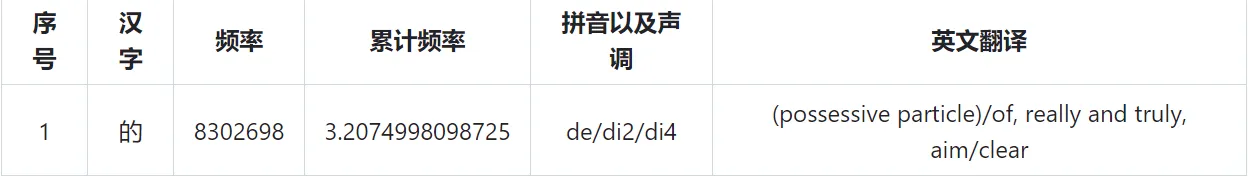
\includegraphics[width=0.7\linewidth]{figures/image5.png}
    \caption{汉字单字字频数据集}
    \label{fig:fig4}
\end{figure}
\begin{enumerate}
    \item \textbf{读取文档内容}\\
  通过 read\_from\_word\_file 函数读取指定的 Word 文件,并将每个段落的文本内容存储在列表中。这个函数调用了 Python docx 库来处理 Word 文档:
    \begin{lstlisting}[caption={读取文档内容实现代码}, label={lst:example}]
  def read_from_word_file(file_path):
      doc = Document(file_path)
      return [para.text for para in doc.paragraphs]
  \end{lstlisting}
    \item \textbf{拼音查找函数}\\
    通过 get\_pinyin 函数从 rare\_char.json 文件中查找指定汉字的拼音,并返回对应的拼音值:
    \begin{lstlisting}[caption={拼音查找函数实现代码}, label={lst:example}]
  def get_pinyin(char, rare_char_data):
      for item in rare_char_data:
          if item['char'] == char:
              return item['pinyin']
      return None  
  \end{lstlisting}
    \item \textbf{处理文本并添加注音}\\
    add\_pinyin\_to\_polyphone\_words 函数负责处理每一段文本,将文本中的多音字和生僻字添加拼音注音:
    \begin{lstlisting}[caption={处理文本并添加注音实现代码}, label={lst:example}]
  def add_pinyin_to_polyphone_words(paragraphs, polyphone_data, rare_char_data):
      polyphonic_chars = {item['char'] for item in polyphone_data}
      rare_chars = {item['char'] for item in rare_char_data}
      output_paragraphs = []
      for paragraph in paragraphs:
          output_paragraph = ""
          char_index = 0
          for char in paragraph:
              if char in rare_chars:
                  output_paragraph += char + '[' + get_pinyin(char, rare_char_data)[0] + ']'
              else:
                  output_paragraph += char
              char_index += 1
          output_paragraphs.append(output_paragraph)
      return output_paragraphs
  \end{lstlisting}
    \item \textbf{主函数:注音处理与文件保存}\\
    pinyin\_nan 函数是主控制函数,它负责从文档中读取文本,处理文本并为多音字和生僻字添加拼音,最后将结果保存到一个新的 Word 文档中。
    \begin{lstlisting}[caption={注音处理与文件保存实现代码}, label={lst:example}]
  def pinyin_nan(input_file='method1/nlp_test.docx', output_doc_path='output_with_pinyin.docx', polyphone='data/polyphone.json', rare_char='data/rare_char.json', level=3000):
      with open(polyphone, 'r', encoding='utf-8') as file:
          polyphone_data = json.load(file)
      with open(rare_char, 'r', encoding='utf-8') as file:
          rare_char_data = json.load(file)
          rare_char_data = rare_char_data[level:]
  
      input_paragraphs_from_word = read_from_word_file(input_file)
      output_paragraphs_with_pinyin = add_pinyin_to_polyphone_words(input_paragraphs_from_word, polyphone_data, rare_char_data)
  
      output_doc = Document()
      for paragraph in output_paragraphs_with_pinyin:
          p = output_doc.add_paragraph(paragraph)
          p.paragraph_format.first_line_indent = Pt(21)  # 设置首行缩进
          for run in p.runs:
              run.font.name = '宋体'
              run.font.size = Pt(12)  # 设置字体大小为小四号(12磅)
  
      output_doc.save(output_doc_path)
  \end{lstlisting}
\end{enumerate}

\subsection{方法三:使用大模型api实现端到端注音}
在这个方法中,我们使用deepseek的大模型api实现端到端的注音功能,
具体的实现方法为:
\begin{itemize}
    \item 传入word文档,使用文档切割工具,按照每100个汉字分成不同的chunks(可以设计不同的切割数量和逻辑)。
    \item 依次将切割好的chunk传入deepseek的"deepseek-chat"模型。
    \item 将大模型api处理的结果记录下来,拼接成一个完整的word文档进行保存。
\end{itemize}
prompt具体来说使用了少样本示例的方法进行提示,激发了模型的能力,我们精心设计的prompt如下:
\begin{itemize}
    \item few\_shots = 行(xíng)人走在路上;我好尴尬(gān)尬(gà)啊
    % \item prompt_gene = "请你在下面的文本中找出多音字和易读错字,并给多音字和易读错字加上拼音和声调,放在圆括号内,让小学三年级学生也能读出,只输出新的文本;例如:{few_shots}.下面是要处理的文本:{text}"
    \item prompt\_gene = 请你在下面的文本中找出多音字和易读错字,并给多音字和易读错字加上拼音和声调,放在圆括号内,让小学三年级学生也能读出,只输出新的文本;例如:\{few\_shots\}.下面是要处理的文本:\{text\}
\end{itemize}
同时我们引入“老师”和“学生”两个检查者,对我们api生成的最后模型进行检查,具体的prompt如下:
\begin{itemize}
    \item prompt\_teacher = 您现在是小学三年的语文老师,擅长给文档标记多音字和易错词读音,请仔细检查以下内容的注音是否正确,给出详细反馈。
    \item prompt\_student = 你现在是小学三年级学生,作业是检查下面的文档请检查以下内容的注音是否正确,并提供简单反馈。
\end{itemize}
我们可以看到,在prompt中,我们可以结合任务场景,在prompt中设计不同年级,进而得到不同的注音效果。
\subsection{UI设计}

\section{小组分工}
\begin{table}[H] % 使用 table 环境并设置浮动选项为 H
    \centering
    \begin{tabular}{>{\centering\arraybackslash}p{0.4\textwidth} >{\centering\arraybackslash}p{0.4\textwidth}} % 设置表格宽度及比例
        \toprule
        \textbf{工作内容} & \textbf{成员名称} \\ % 表头
        \midrule
        method1代码实现 & 张志成 \\
        method2代码实现 & 张志成,江震南,左斌斌 \\
        method3代码实现 & 郝锐,邱骏坤 \\
        难字实现 & 左斌斌,孟鑫攀 \\
        UI实现 & 曾楠馨,沙霖 \\
        报告撰写 & 朱英健,黄少平 \\
        PPT制作与汇报展示 & 柏天佑 \\
        测试与量化指标 & 江震南,龚子俊 \\
        \bottomrule
    \end{tabular}
    \caption{工作内容与成员名称}
    \label{tab:work_distribution}
\end{table}

%%----------- 参考文献 -------------------%%
%在reference.bib文件中填写参考文献,此处自动生成

% \reference


\end{document}